\chapter{Standardization efforts}

\vspace{1cm}

Markdown achieved its objectives of readability and simplicity, which were the main arguments for its fast rise in popularity.
What started as a simple Perl script that converts Markdown to HTML via regex replacements became a phenomenon, and was adopted in many
famous online services and pieces of software. However, there is no real ``specification'' for Markdown beyond the original blog post
introducing the language and a few other pages on Gruber's website.\footcite{gruber2004markdown}
With time, one of Markdown's strengths, it's simplicity, also became one of its flaws for a few reasons:

\begin{itemize}
    \item While integrating Markdown, many developers realised that unfortunately Markdown is filled with unintentional errors
    and breaking states, which generate invalid HTML.
    \item Lack of features
    \item Other output formats other than HTML were often requested, chiefly PDF.
\end{itemize}

This led to various implementations and syntaxes appearing all over the web-space, all of them incompatible with each other
(see REF NEXT CHAP HERE).\newline

Indeed, even extremely simple examples lead to several different HTML outputs depending on the type of implementation used to
interpret the markdown snippet. On figure \ref{fig:babelmark}, we see a simple example of a markdown text: two headings of
level 1 and 2, with no other text. Even a simple example as that leads to six different HTML outputs (three are shown in the figure).

\begin{figure}[H]
\centering
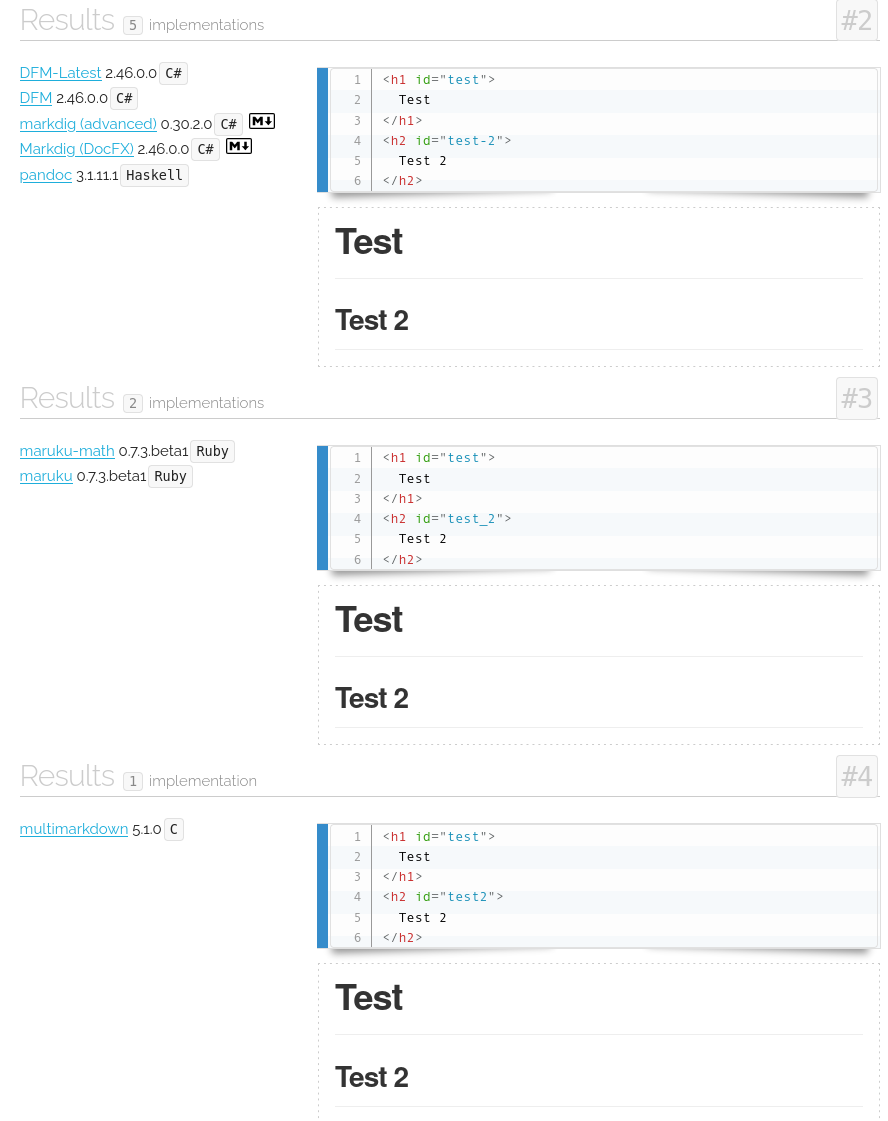
\includegraphics[scale=0.3]{babelmark}
\caption{Babelmark listing some of many possible outputs from markdown implementations}
\label{fig:babelmark}
\end{figure}

---

TODO:

Discuss CommonMark

---

\cite{leonard2016text}